\section{Problem Formulation} \label{sec:probform}  

We study systems of quadratic equations of the form
\begin{align}
& Q(\vx)+L\vx=\vu\label{eq:Quad}
\end{align}
where $Q: \mathbb{R}^n \mapsto \mathbb{R}^n$ is a vector-valued quadratic function, that is, there exist matrices $Q_1,\ldots,Q_n $ $\in \mathbb{R}^{n\times n}$, such that
\[[Q(\vx)]_i = \vx^T Q_{i} \vx \quad \forall i \in [n]\]
and $L \in \mathbb{R}^{n\times n}$, $\vu \in \mathbb{R}^n$. 
We are interested in solutions to this system of equations under linear constraints of the form
\begin{align}
(A\vx)_i\leq b_i \quad \forall i \in [n]\label{eq:xLimits}
\end{align}
However, the parameter $\vu$ is uncertain and only known up to certain error bounds
\begin{align}
u^{\min}_i=u_i^*-e_i \leq u_i \leq =u_i^*+e_i=u^{\max}_i \quad \forall i \in [n] \label{eq:uLimits}
\end{align}
where $\vu^*$ is a forecast for $\vu$ and $\ve$ denotes the error bounds associated with the forecast. 
For example, in the case of quadratic equations appearing in infrastructure networks like the power grid, $u_i$ represents uncertain power generation or consumption (for example uncertain weather-dependent power sources like solar or wind power). 
In the case of stochastic processes, $\vu^*$ represents an initial state distribution.

\begin{cdef}[Robust Feasibility and Robust Margin problem]  \label{RobustDef}
Determine whether for all values of $\vu$ satisfying \eqref{eq:uLimits}, the system of equations \eqref{eq:Quad} has a solution lying within the interior of the set of all  $\vx$ satisfying the constraints in \eqref{eq:xLimits}. 
If this is true, the system comprised of \eqref{eq:Quad},\eqref{eq:xLimits},\eqref{eq:uLimits} is said to be \emph{robust feasible}. 
The largest $r$ such that $e_i\geq r \ \forall i~$ such that $~e_i>0$ in \eqref{eq:uLimits} such that the system is robust feasible is said to be the \emph{robustness margin}. 
See \cref{fig:RFeas} for a pictorial depiction. 
\end{cdef}

\begin{figure}[htp!]
\begin{center}
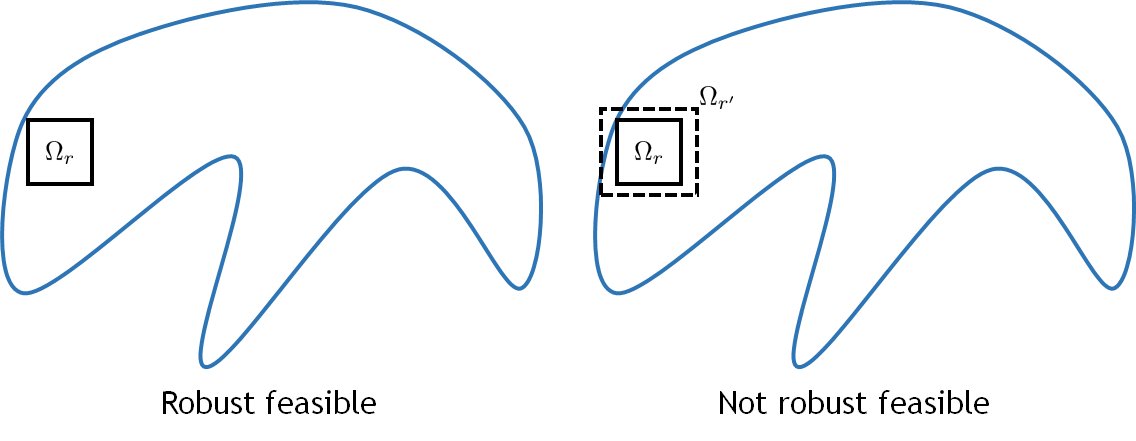
\includegraphics[scale=1.1, bb=0in 0in 5in 2in]{Figures/RobFeas.png} % {Figures/Rfeas}
\end{center}
\caption{Illustration of robust feasibility.
The system is robust feasible at the level of $r$ (left), but is not robust feasible at $r' > r$ (right).}
\label{fig:RFeas}
\end{figure}

The definition for robustness margin is left here in its most general form so as to capture all scenarios under which a researcher may find themselves. 
For instance it very well may be the case that only some of the dimensions of $\vu$ will have margins of uncertainty. 
Furthermore, one may have need of computing the robustness margin for only a subset of the dimensions of $\vu$ which pertain to problem areas or nodes of particular interest to the research. 
This manual restriction will of course produce a robustness margin greater than or equal to that obtained by considering all dimensions, which certainly remains an option under the current setting. 
